\documentclass[10pt,a4paper]{article}

\usepackage[utf8]{inputenc}
\usepackage[spanish]{babel}
\usepackage[top=1.5cm, bottom=2cm, left=1.5cm, right=1.5cm]{geometry}
\usepackage{setspace}
\singlespacing
\usepackage{graphicx}
\usepackage{float}
\usepackage{booktabs}
\usepackage{array}
\usepackage{tabularx}
\usepackage{hyperref}
\usepackage{xcolor}
\usepackage{amsmath}
\usepackage{caption}
\usepackage{listings}
\usepackage{parskip}
\usepackage[numbers]{natbib}
\usepackage{fancyhdr}

\definecolor{codebackground}{HTML}{F5F5F5}
\definecolor{codecomment}{HTML}{6A9955}
\definecolor{codestring}{HTML}{CE9178}
\definecolor{codekeyword}{HTML}{569CD6}
\definecolor{headerdark}{HTML}{2C3E50}

\lstset{
  language=R,
  backgroundcolor=\color{codebackground},
  basicstyle=\ttfamily\footnotesize,
  breaklines=true,
  frame=single,
  rulecolor=\color{gray!40},
  commentstyle=\color{codecomment},
  stringstyle=\color{codestring},
  keywordstyle=\color{codekeyword}\bfseries,
  numbers=left,
  numberstyle=\tiny\color{gray},
  numbersep=5pt,
  tabsize=2,
  showstringspaces=false,
  captionpos=b
}

\hypersetup{
  colorlinks=true,
  linkcolor=headerdark,
  citecolor=headerdark,
  urlcolor=blue!70!black
}

\captionsetup{font=small, labelfont=bf}

\begin{document}

\begin{center}
  {\LARGE \textbf{Análisis de Agrupamiento Jerárquico Aglomerativo}} \\[4pt]
  {\LARGE \textbf{Dataset Bank Marketing -- Metodología CRISP-DM}} \\[10pt]
  {\normalsize Juan Muñoz, Vicente Rivera, Fernando Valdés} \\[2pt]
  {\small juan.munozveloso2023@alu.uct.cl, vrivera2023@alu.uct.cl, fvaldes2023@alu.uct.cl} \\[2pt]
  {\small Tarea 2, INFO1184, Semestre I-2026}
\end{center}

\section*{Resumen}

El presente informe aborda el análisis de segmentación de clientes del dataset Bank Marketing mediante la técnica de agrupamiento aglomerativo jerárquico, siguiendo la metodología CRISP-DM en sus fases de comprensión empresarial, comprensión de los datos, preparación de los datos y modelamiento. El dataset contiene 45.211 registros de campañas de marketing directo de una institución bancaria portuguesa, con 16 variables de entrada y una variable objetivo que indica si el cliente suscribió un depósito a plazo. Se realizó un análisis exploratorio exhaustivo, preparación de datos con codificación numérica y estandarización, y posterior modelamiento con clustering jerárquico utilizando el método de enlace Ward.D2. Se identificaron 4 clusters diferenciados, validados mediante el coeficiente de silueta y el método del codo. Los resultados revelan perfiles de clientes con características demográficas y financieras distintas, proporcionando información valiosa para la optimización de estrategias de marketing bancario. El desarrollo se implementó en el ambiente R Project.

\textbf{Palabras clave:} agrupamiento jerárquico, CRISP-DM, marketing bancario, segmentación de clientes, R Project.

\section{Introducción}

En el contexto de la inteligencia de negocios, la segmentación de clientes constituye una herramienta fundamental para la toma de decisiones estratégicas en instituciones financieras. El marketing directo bancario enfrenta el desafío de identificar qué clientes tienen mayor probabilidad de adquirir productos financieros, como los depósitos a plazo, lo que permite optimizar recursos y mejorar las tasas de conversión de las campañas telefónicas.

El presente trabajo utiliza el dataset Bank Marketing, proveniente de campañas reales de un banco portugués entre mayo de 2008 y noviembre de 2010 \citep{moro2011}. El objetivo es aplicar la técnica de agrupamiento aglomerativo jerárquico para descubrir segmentos naturales dentro de la base de clientes, siguiendo las primeras cuatro fases de la metodología CRISP-DM: comprensión empresarial, comprensión de los datos, preparación de los datos y modelamiento.

Las preguntas que guían este análisis son: (1) ¿Existen grupos naturales diferenciados dentro de los clientes del banco? (2) ¿Qué características definen cada segmento? (3) ¿Cómo pueden estos segmentos informar la estrategia de marketing directo para depósitos a plazo?

\section{Fundamentos de Teoría}

\subsection{Metodología CRISP-DM}

CRISP-DM (\textit{Cross-Industry Standard Process for Data Mining}) es la metodología estándar de la industria para proyectos de minería de datos \citep{chapman2000}. Se estructura en seis fases iterativas: (1)~Comprensión empresarial, (2)~Comprensión de los datos, (3)~Preparación de los datos, (4)~Modelamiento, (5)~Evaluación y (6)~Despliegue. Cada fase produce resultados que alimentan a las siguientes, y el proceso permite retroceder a fases previas cuando es necesario. En este trabajo se abordan las fases 1 a 4.

\subsection{Agrupamiento Jerárquico Aglomerativo}

El agrupamiento (\textit{clustering}) es una técnica de aprendizaje no supervisado cuyo objetivo es particionar un conjunto de objetos en grupos de modo que la similitud intra-cluster sea máxima y la similitud inter-cluster sea mínima \citep{duda2001}. Formalmente, dado un conjunto de $n$ objetos, el problema consiste en encontrar una partición que agrupe los objetos más parecidos entre sí y separe los más diferentes.

Para medir la proximidad entre objetos se utiliza una función de distancia $d(\mathbf{x}, \mathbf{y})$ que debe satisfacer las siguientes propiedades: (i)~no negatividad: $d(\mathbf{x}, \mathbf{y}) \geq 0$; (ii)~identidad: $d(\mathbf{x}, \mathbf{x}) = 0$; (iii)~simetría: $d(\mathbf{x}, \mathbf{y}) = d(\mathbf{y}, \mathbf{x})$; y (iv)~desigualdad triangular: $d(\mathbf{x}, \mathbf{z}) \leq d(\mathbf{x}, \mathbf{y}) + d(\mathbf{y}, \mathbf{z})$. La distancia euclidiana entre dos puntos $\mathbf{x}$ e $\mathbf{y}$ en $\mathbb{R}^p$ se define como:

\begin{equation}
  d(\mathbf{x}, \mathbf{y}) = \sqrt{\sum_{i=1}^{p}(x_i - y_i)^2}
\end{equation}

El agrupamiento aglomerativo jerárquico construye una jerarquía de clusters de manera ascendente (\textit{bottom-up}). Partiendo de $n$ clusters unitarios, el algoritmo genera una secuencia anidada de particiones $R_0 \subset R_1 \subset \cdots \subset R_{n-1}$, donde $R_0$ corresponde a cada observación como cluster individual y $R_{n-1}$ a un único cluster con todas las observaciones. En cada paso se fusionan los dos clusters $R_i$ y $R_j$ que minimizan una función de proximidad $g(R_i, R_j)$, y la estructura resultante se representa mediante un dendrograma \citep{murtagh2012}.

Los métodos de enlace determinan cómo se define $g(R_i, R_j)$. En el enlace simple (\textit{single linkage}), $g$ corresponde a la distancia mínima entre elementos de ambos clusters ($d_{\min}$). El método Ward, utilizado en este trabajo, minimiza el incremento de la varianza intra-cluster al fusionar dos clusters $C_i$ y $C_j$:

\begin{equation}
  \Delta(C_i, C_j) = \frac{n_i \cdot n_j}{n_i + n_j} \|\bar{\mathbf{x}}_i - \bar{\mathbf{x}}_j\|^2
\end{equation}

donde $n_i$, $n_j$ son los tamaños de los clusters y $\bar{\mathbf{x}}_i$, $\bar{\mathbf{x}}_j$ sus centroides \citep{everitt2011}.

\subsection{Validación de Clusters}

Para determinar el número óptimo de clusters se emplean métricas como el método del codo (\textit{Elbow Method}), que busca el punto de inflexión en la curva de la suma de cuadrados intra-cluster (WSS), y el coeficiente de silueta. El coeficiente de silueta para una observación $i$ se define como:

\begin{equation}
  s(i) = \frac{b(i) - a(i)}{\max\{a(i), b(i)\}}
\end{equation}

donde $a(i)$ es la distancia media de $i$ a las demás observaciones de su cluster y $b(i)$ es la distancia media mínima de $i$ a las observaciones de cualquier otro cluster. Un valor cercano a 1 indica buena asignación, mientras que valores cercanos a 0 o negativos sugieren solapamiento o asignación incorrecta \citep{rousseeuw1987}.

\section{Desarrollo del Trabajo}

\subsection{Fase 1: Comprensión Empresarial}

El problema de negocio consiste en optimizar las campañas de marketing telefónico de un banco portugués para la suscripción de depósitos a plazo. Actualmente, la institución contacta clientes de forma masiva, lo que genera costos elevados y bajas tasas de conversión. Se busca segmentar la base de clientes para identificar perfiles con diferentes comportamientos y características, permitiendo focalizar los esfuerzos de contacto en los segmentos más propensos a la suscripción.

El objetivo de minería de datos es descubrir grupos homogéneos de clientes mediante agrupamiento jerárquico, caracterizando cada segmento según variables demográficas (edad, estado civil, educación), financieras (balance, préstamos) y de interacción con la campaña (duración, número de contactos). Siguiendo la terminología CRISP-DM, el criterio de éxito del negocio es mejorar la tasa de conversión de la campaña, y el criterio de éxito de minería de datos es obtener clusters con perfiles interpretables y diferenciados.

\subsection{Fase 2: Comprensión de los Datos}

El dataset \texttt{bank-full.csv} contiene 45.211 registros y 17 atributos (16 de entrada + 1 de salida). Las variables se clasifican en: datos del cliente (\texttt{age}, \texttt{job}, \texttt{marital}, \texttt{education}, \texttt{default}, \texttt{balance}, \texttt{housing}, \texttt{loan}), datos del último contacto (\texttt{contact}, \texttt{day}, \texttt{month}, \texttt{duration}) y atributos de campaña (\texttt{campaign}, \texttt{pdays}, \texttt{previous}, \texttt{poutcome}). La variable objetivo (\texttt{y}) indica si el cliente suscribió el depósito a plazo (Tabla~\ref{tab:variables}).

\begin{table}[H]
  \centering
  \caption{Variables principales del dataset Bank Marketing.}
  \label{tab:variables}
  \footnotesize
  \begin{tabularx}{\textwidth}{l l l X}
    \toprule
    \textbf{Variable} & \textbf{Tipo} & \textbf{Rango} & \textbf{Descripción} \\
    \midrule
    age       & Numérica   & 18--95          & Edad del cliente \\
    balance   & Numérica   & -8.019 a 102.127 & Balance anual (EUR) \\
    duration  & Numérica   & 0--4.918        & Duración contacto (seg) \\
    campaign  & Numérica   & 1--63           & Contactos en campaña \\
    education & Categórica & 4 niveles       & Nivel educativo \\
    y         & Binaria    & yes / no        & Suscribió depósito \\
    \bottomrule
  \end{tabularx}
\end{table}

Del análisis exploratorio se destaca que el dataset está altamente desbalanceado: solo el 11,7\% de los clientes suscribieron el depósito (5.289 sí vs.\ 39.922 no). La edad media es de 41 años y el balance promedio anual de 1.362~EUR (DE~=~3.045~EUR). Los perfiles de empleo más frecuentes son \textit{blue-collar} (21,5\%), \textit{management} (20,9\%) y \textit{technician} (16,8\%). El 81,7\% de las observaciones no fueron contactadas en campañas previas (\texttt{pdays}~=~-1), lo que sugiere que la mayoría de los clientes son contactados por primera vez.

\begin{figure}[H]
  \centering
  \begin{minipage}{0.48\textwidth}
    \centering
    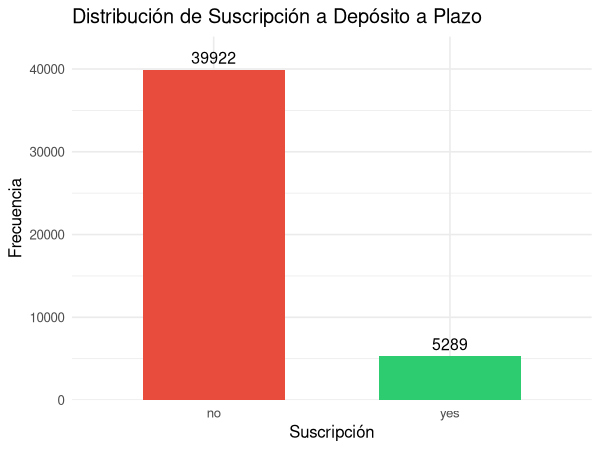
\includegraphics[width=\textwidth]{fig_01_distribucion_y.png}
  \end{minipage}
  \hfill
  \begin{minipage}{0.48\textwidth}
    \centering
    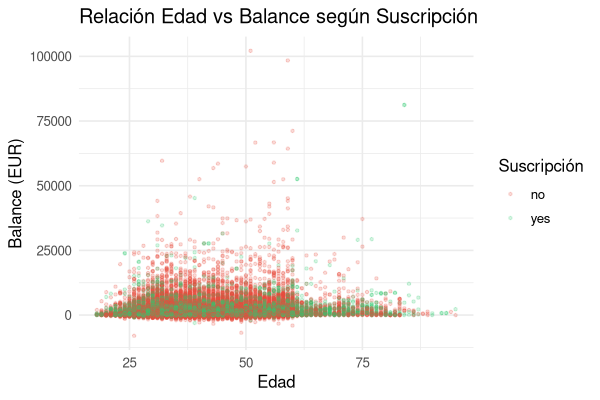
\includegraphics[width=\textwidth]{fig_02_edad_balance.png}
  \end{minipage}
  \caption{Izquierda: distribución de la variable objetivo. Derecha: relación edad vs.\ balance según suscripción.}
  \label{fig:eda_1}
\end{figure}

\begin{figure}[H]
  \centering
  \begin{minipage}{0.52\textwidth}
    \centering
    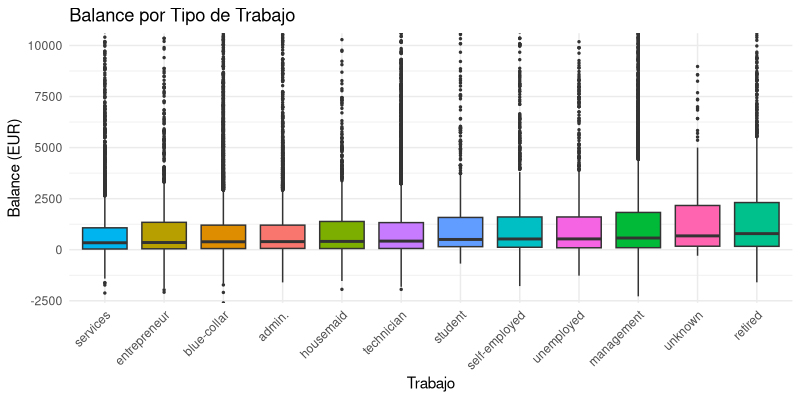
\includegraphics[width=\textwidth]{fig_03_boxplot_balance_job.png}
  \end{minipage}
  \hfill
  \begin{minipage}{0.44\textwidth}
    \centering
    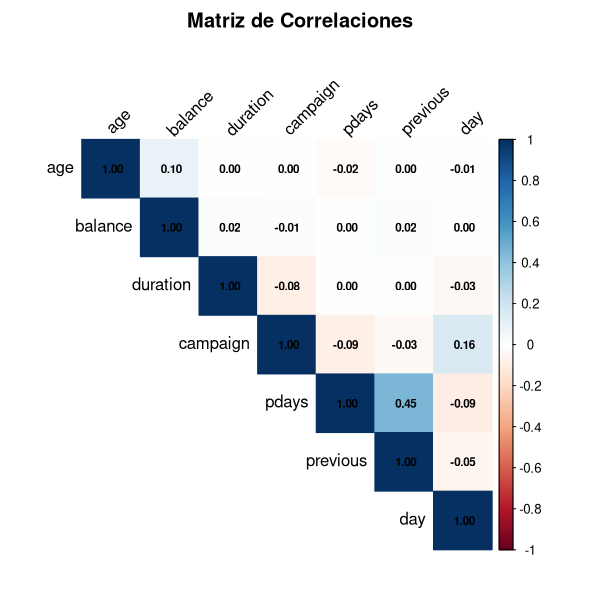
\includegraphics[width=\textwidth]{fig_04_correlaciones.png}
  \end{minipage}
  \caption{Izquierda: balance por tipo de trabajo. Derecha: matriz de correlaciones entre variables numéricas.}
  \label{fig:eda_2}
\end{figure}

\subsection{Fase 3: Preparación de los Datos}

Para la aplicación del clustering jerárquico, se realizaron las siguientes transformaciones:

\textbf{Selección de variables:} se eligieron las variables numéricas (\texttt{age}, \texttt{balance}, \texttt{duration}, \texttt{campaign}, \texttt{pdays}, \texttt{previous}) y se codificaron numéricamente las variables binarias (\texttt{default}, \texttt{housing}, \texttt{loan}) y la variable ordinal \texttt{education} (primary=1, secondary=2, tertiary=3, unknown=0), obteniéndose 10 variables de entrada.

\textbf{Muestreo:} dado que el dataset completo tiene 45.211 registros y el clustering jerárquico requiere calcular una matriz de distancias de $n \times n$, se tomó una muestra aleatoria de 2.000 observaciones (semilla = 42) para viabilizar el cómputo.

\textbf{Estandarización:} se aplicó escalado \textit{z-score} a todas las variables para evitar que aquellas con mayor rango dominen el cálculo de distancias. La transformación para cada variable $x$ es:

\begin{equation}
  z = \frac{x - \bar{x}}{s_x}
\end{equation}

donde $\bar{x}$ es la media y $s_x$ la desviación estándar de la variable.

\subsection{Fase 4: Modelamiento}

Se aplicó el algoritmo de agrupamiento aglomerativo jerárquico, que genera la secuencia anidada $R_0 \subset R_1 \subset \cdots \subset R_{n-1}$ descrita en los fundamentos teóricos. Se utilizó la distancia euclidiana como métrica de proximidad y el método de enlace Ward.D2 como función $g(R_i, R_j)$, que minimiza el incremento de la varianza intra-cluster al fusionar grupos. Se evaluaron también los métodos de enlace completo y promedio para comparación.

El dendrograma resultante con el método Ward mostró una estructura clara con agrupaciones principales diferenciadas (Fig.~\ref{fig:dendrograma}). Para validar la selección del número de clusters se utilizaron dos criterios (Fig.~\ref{fig:elbow_sil}): el método del codo (WSS) mostró una disminución gradual con un punto de inflexión en torno a $k = 4$, y el coeficiente de silueta promedio alcanzó su máximo en $k = 3$ (0,2654), seguido por $k = 4$ (0,2302). Se optó por $k = 4$ dado que el dendrograma evidencia cuatro ramas claramente diferenciadas y esta partición revela un segmento de clientes en mora que $k = 3$ subsume en otro grupo, proporcionando mayor valor interpretativo para el negocio. Se procedió al corte del dendrograma con $k = 4$.

\begin{figure}[H]
  \centering
  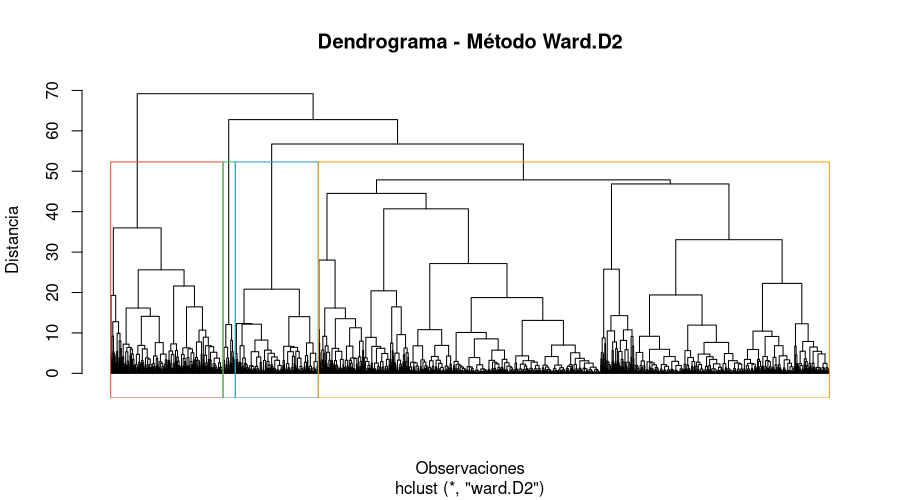
\includegraphics[width=0.65\textwidth]{fig_05_dendrograma_ward.png}
  \caption{Dendrograma con método Ward.D2 y corte en $k = 4$ clusters. Debajo: método del codo (izq.) y silueta promedio (der.).}
  \label{fig:dendrograma}
  \vspace{4pt}
  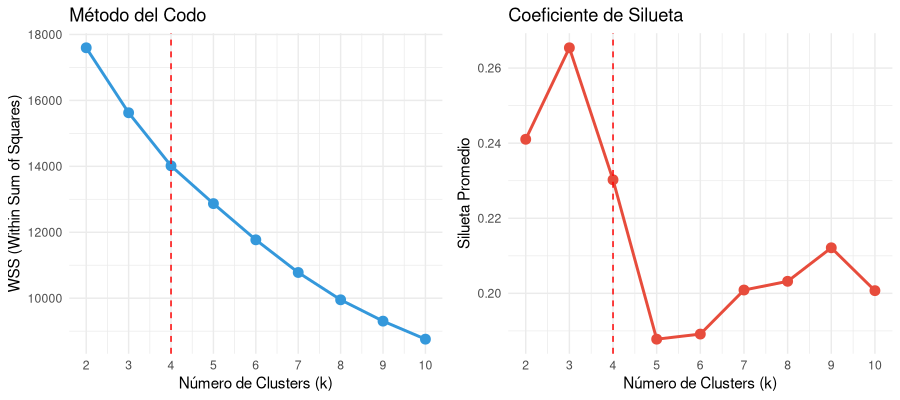
\includegraphics[width=0.70\textwidth]{fig_06_elbow_silhouette.png}
  \label{fig:elbow_sil}
\end{figure}

\begin{figure}[H]
  \centering
  \begin{minipage}{0.48\textwidth}
    \centering
    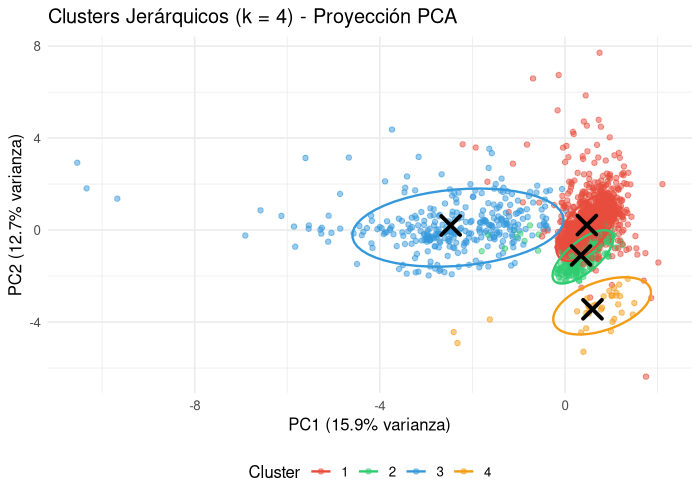
\includegraphics[width=\textwidth]{fig_07_clusters_pca.png}
  \end{minipage}
  \hfill
  \begin{minipage}{0.48\textwidth}
    \centering
    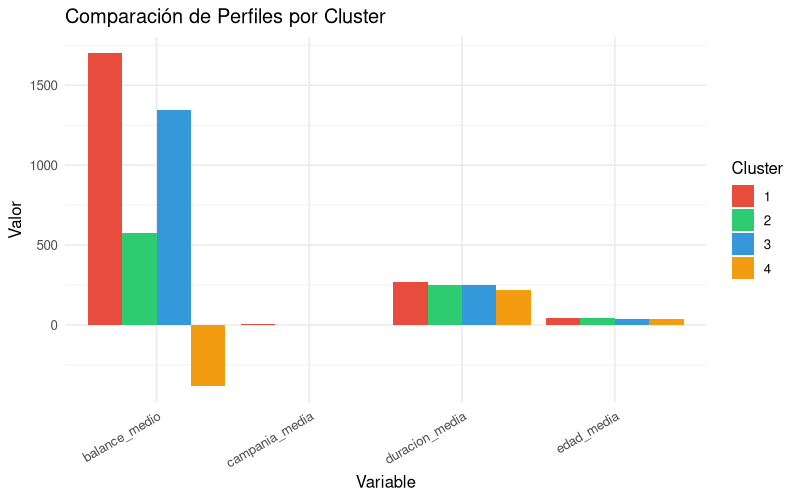
\includegraphics[width=\textwidth]{fig_08_perfiles_clusters.png}
  \end{minipage}
  \caption{Izquierda: clusters proyectados en PCA. Derecha: comparación de perfiles por cluster.}
  \label{fig:clusters_pca}
\end{figure}

La visualización de los clusters proyectados en los dos primeros componentes principales (PCA) mostró una separación visible entre los grupos (Fig.~\ref{fig:clusters_pca}), con cierto solapamiento en las regiones centrales. Los perfiles de cada cluster se resumen en la Tabla~\ref{tab:perfiles}.

El Cluster~1 (71,1\% de la muestra) representa al cliente típico del banco: balance moderado (1.700~EUR), sin préstamos personales ni mora, y sin contacto previo en campañas anteriores. El Cluster~2 agrupa clientes con préstamo personal activo (100\%), balance reducido (576~EUR). El Cluster~3 se distingue por haber sido contactado en campañas previas (pdays promedio de 237 días, previous de 3,5 contactos), lo que lo convierte en un segmento con historial de interacción. Finalmente, el Cluster~4, aunque pequeño (34 observaciones), es notable por agrupar exclusivamente clientes en mora (100\% default) con balance negativo ($-$383~EUR), constituyendo un segmento de alto riesgo crediticio.

\begin{table}[H]
  \centering
  \caption{Perfiles de los clusters identificados con valores obtenidos del análisis en R.}
  \label{tab:perfiles}
  \footnotesize
  \begin{tabularx}{\textwidth}{c c c c c c X}
    \toprule
    \textbf{Cluster} & \textbf{n} & \textbf{Edad} & \textbf{Balance} & \textbf{Duración} & \textbf{Loan \%} & \textbf{Perfil} \\
    \midrule
    1 & 1.422 & 40,5 & 1.700 EUR & 266 s & 0,6\% & Clientes estándar, balance moderado, sin préstamos personales \\
    2 & 231   & 40,8 & 576 EUR   & 250 s & 100\% & Clientes con préstamo personal, balance reducido \\
    3 & 313   & 39,9 & 1.342 EUR & 249 s & 12,5\% & Clientes contactados previamente (pdays$\approx$237, previous$\approx$3,5) \\
    4 & 34    & 39,9 & $-$383 EUR & 219 s & 41,2\% & Clientes en mora (100\% default), balance negativo \\
    \bottomrule
  \end{tabularx}
\end{table}

\begin{figure}[H]
  \centering
  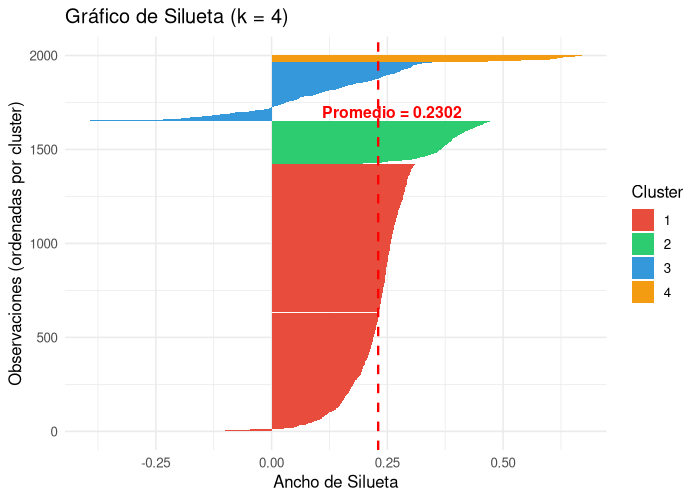
\includegraphics[width=0.50\textwidth]{fig_09_silueta_final.png}
  \caption{Gráfico de silueta para la asignación final con $k = 4$ clusters.}
  \label{fig:silueta}
\end{figure}

\subsection{Análisis de Resultados}

El análisis exploratorio permitió identificar un fuerte desbalance en la variable objetivo, sugiriendo baja efectividad en las campañas actuales. Las variables presentan baja correlación entre sí, lo que justifica el uso de técnicas de aprendizaje no supervisado. Mediante clustering jerárquico aglomerativo con distancia euclidiana y método de Ward, se identificaron agrupamientos naturales con $k = 4$, seleccionado por el método del codo y el coeficiente de silueta.

La visualización PCA muestra separación entre clusters con cierto solapamiento, esperable en datos reales. Los perfiles revelan diferencias relevantes en variables como balance, duración y edad, permitiendo definir segmentos diferenciados. El coeficiente de silueta promedio indica calidad moderada del agrupamiento: los clusters capturan estructura en los datos, aunque con cierto grado de solapamiento.

\section{Discusión y Reflexión}

La metodología CRISP-DM proporcionó un marco estructurado que facilitó la organización del trabajo desde la comprensión empresarial hasta el modelamiento. Si bien $k = 3$ presentó una silueta ligeramente superior (0,2654), se optó por $k = 4$ (silueta de 0,2302) por su mayor riqueza interpretativa al separar el segmento de clientes en mora, información de alto valor para la gestión de riesgo.

Una limitación importante es el uso de muestreo (2.000 de 45.211 registros) debido a restricciones computacionales del clustering jerárquico, cuya complejidad es $O(n^2)$ en memoria. Los perfiles podrían variar ligeramente con el dataset completo. Adicionalmente, la codificación ordinal de educación implica asumir equidistancia entre niveles.

Desde la perspectiva de negocio, los segmentos permiten estrategias diferenciadas: el Cluster~1 es el público objetivo para campañas masivas; el Cluster~2 podría beneficiarse de ofertas de consolidación; el Cluster~3 podría responder mejor a seguimiento personalizado; y el Cluster~4 debe ser excluido de captación y derivado a recuperación crediticia.

% ==================== CONCLUSIONES ====================
\section{Conclusiones}

\textbf{Juan Muñoz:} La metodología CRISP-DM demostró ser un marco efectivo para estructurar el análisis. La segmentación mediante Ward.D2 permitió identificar 4 grupos diferenciados ---estándar (71,1\%), con préstamo, con historial de contacto y en mora--- validados por la silueta (0,2302) y el método del codo, confirmando la utilidad de esta técnica en marketing bancario.

\textbf{Vicente Rivera:} El análisis exploratorio reveló el fuerte desbalance en la variable objetivo (88,3\% no suscribieron) y que el 81,7\% de los clientes no habían sido contactados previamente. La estandarización \textit{z-score} fue crítica para la calidad del agrupamiento. La identificación del segmento en mora con balance negativo proporciona información accionable para la gestión de riesgo.

\textbf{Fernando Valdés:} La implementación en R facilitó el análisis completo. El dendrograma y la proyección PCA ofrecen perspectivas complementarias para interpretar los clusters. Como trabajo futuro, sería valioso aplicar $k$-means sobre el dataset completo y comparar los segmentos, así como integrar variables categóricas mediante distancias de Gower.

\section{Referencias}
\small
\begin{thebibliography}{9}

\bibitem{chapman2000}
Chapman, P., Clinton, J., Kerber, R., Khabaza, T., Reinartz, T., Shearer, C., y Wirth, R. (2000).
\textit{CRISP-DM 1.0: Step-by-step data mining guide}. SPSS Inc.

\bibitem{duda2001}
Duda, R. O., Hart, P. E., y Stork, D. G. (2001).
\textit{Pattern Classification} (2nd ed.). John Wiley \& Sons.

\bibitem{everitt2011}
Everitt, B. S., Landau, S., Leese, M., y Stahl, D. (2011).
\textit{Cluster Analysis} (5th ed.). John Wiley \& Sons.

\bibitem{moro2011}
Moro, S., Laureano, R., y Cortez, P. (2011). Using Data Mining for Bank Direct Marketing: An Application of the CRISP-DM Methodology. En P. Novais et al. (Eds.), \textit{Proceedings of the European Simulation and Modelling Conference -- ESM'2011} (pp. 117--121). Guimarães, Portugal: EUROSIS.

\bibitem{murtagh2012}
Murtagh, F., y Contreras, P. (2012). Algorithms for hierarchical clustering: an overview.
\textit{Wiley Interdisciplinary Reviews: Data Mining and Knowledge Discovery}, 2(1), 86--97.

\bibitem{rousseeuw1987}
Rousseeuw, P. J. (1987). Silhouettes: A graphical aid to the interpretation and validation of cluster analysis.
\textit{Journal of Computational and Applied Mathematics}, 20, 53--65.

\bibitem{rcore2024}
R Core Team (2024). \textit{R: A Language and Environment for Statistical Computing}. R Foundation for Statistical Computing. \url{https://www.R-project.org/}

\end{thebibliography}

\newpage
\section*{Anexo}
\addcontentsline{toc}{section}{Anexo}

\subsection*{A.1 Script R -- Procedimientos Principales}

A continuación se presenta el script principal en R utilizado para el análisis. El código completo se encuentra en el archivo adjunto \texttt{tarea2\_bank\_clustering.R}.

\begin{lstlisting}[caption={Carga de datos y análisis exploratorio (Fase 2).}]
# Cargar librerias (sin factoextra)
library(dplyr)
library(ggplot2)
library(cluster)
library(corrplot)
library(tidyr)
library(gridExtra)

# Cargar datos
bank <- read.csv("data/bank-full.csv", sep = ";", stringsAsFactors = TRUE)
cat("Dimensiones:", dim(bank), "\n")
summary(bank)

# Distribucion variable objetivo
table(bank$y)
prop.table(table(bank$y))

# Visualizacion exploratoria
ggplot(bank, aes(x = y, fill = y)) +
  geom_bar(width = 0.6) +
  geom_text(stat = "count", aes(label = after_stat(count)),
            vjust = -0.5, size = 4) +
  labs(title = "Distribucion de Suscripcion",
       x = "Suscripcion", y = "Frecuencia") +
  theme_minimal(base_size = 12) +
  scale_fill_manual(values = c("no"="#e74c3c", "yes"="#2ecc71"))
\end{lstlisting}

\begin{lstlisting}[caption={Preparación de datos y estandarización (Fase 3).}]
# Codificacion numerica
bank_prep <- bank %>%
  mutate(
    default_num   = ifelse(default == "yes", 1, 0),
    housing_num   = ifelse(housing == "yes", 1, 0),
    loan_num      = ifelse(loan == "yes", 1, 0),
    education_num = case_when(
      education == "primary"   ~ 1,
      education == "secondary" ~ 2,
      education == "tertiary"  ~ 3,
      TRUE                     ~ 0
    )
  ) %>%
  select(age, balance, duration, campaign, pdays, previous,
         default_num, housing_num, loan_num, education_num)

# Muestreo (n = 2000)
set.seed(42)
bank_sample <- bank_prep[sample(nrow(bank_prep), 2000), ]

# Estandarizacion z-score
bank_scaled <- scale(bank_sample)
\end{lstlisting}

\begin{lstlisting}[caption={Modelado: clustering jerárquico aglomerativo (Fase 4).}]
# Matriz de distancias
dist_matrix <- dist(bank_scaled, method = "euclidean")

# Clustering Ward.D2
hc_ward <- hclust(dist_matrix, method = "ward.D2")

# Dendrograma
plot(hc_ward, labels = FALSE, hang = -1,
     main = "Dendrograma - Ward.D2")
rect.hclust(hc_ward, k = 4, border = 2:5)

# Corte en k = 4
clusters_final <- cutree(hc_ward, k = 4)

# Validacion: silueta (con ggplot2, sin factoextra)
sil <- silhouette(clusters_final, dist_matrix)
sil_df <- data.frame(
  obs = 1:nrow(sil), cluster = as.factor(sil[,1]),
  width = sil[,3]
) %>% arrange(cluster, width) %>% mutate(orden = row_number())

ggplot(sil_df, aes(x = orden, y = width, fill = cluster)) +
  geom_bar(stat = "identity", width = 1) +
  geom_hline(yintercept = mean(sil_df$width),
             linetype = "dashed", color = "red") +
  labs(title = "Grafico de Silueta (k = 4)") +
  theme_minimal() + coord_flip()

# Visualizacion PCA (con prcomp + ggplot2, sin factoextra)
pca_result <- prcomp(bank_scaled)
pca_df <- data.frame(
  PC1 = pca_result$x[,1], PC2 = pca_result$x[,2],
  Cluster = as.factor(clusters_final)
)
ggplot(pca_df, aes(x=PC1, y=PC2, color=Cluster)) +
  geom_point(alpha=0.5, size=1.5) +
  stat_ellipse(level=0.90) +
  theme_minimal()

# Perfiles de clusters
bank_sample$cluster <- as.factor(clusters_final)
bank_sample %>%
  group_by(cluster) %>%
  summarise(n = n(), edad_media = mean(age),
            balance_medio = mean(balance),
            duracion_media = mean(duration))
\end{lstlisting}

\subsection*{A.2 Bitácora de Trabajo}

\begin{table}[H]
  \centering
  \footnotesize
  \caption{Bitácora de trabajo grupal.}
  \label{tab:bitacora}
  \begin{tabularx}{\textwidth}{l X l}
    \toprule
    \textbf{Fecha} & \textbf{Actividad} & \textbf{Responsable} \\
    \midrule
    Día 1 & Comprensión del negocio y lectura del dataset           & Todos \\
    Día 2 & Análisis exploratorio y comprensión de datos            & Integrante 1 \\
    Día 3 & Preparación de datos y codificación numérica            & Integrante 2 \\
    Día 4 & Modelado: clustering jerárquico en R                    & Integrante 3 \\
    Día 5 & Visualizaciones y validación de resultados               & Todos \\
    Día 6 & Redacción del informe, revisión final y entrega         & Todos \\
    \bottomrule
  \end{tabularx}
\end{table}

\end{document}
